\section{Memory Inspection Window}
The memory inspection window is used to inspect the physical memory and the cache of the emulator.

\begin{figure}[H]
\begin{center}
	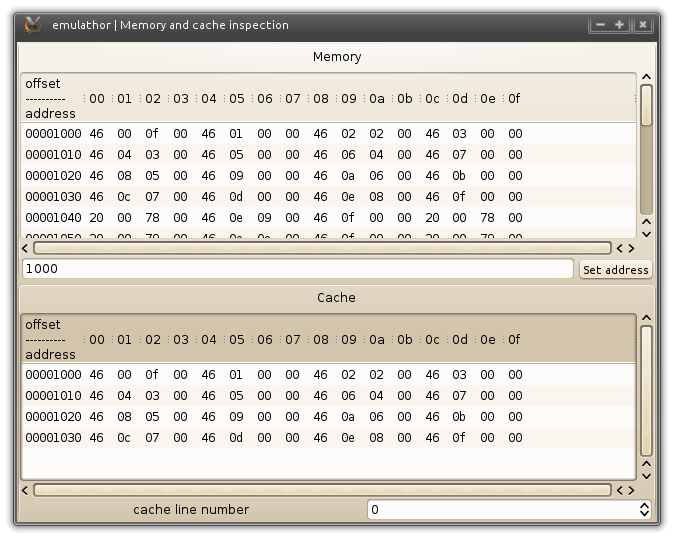
\includegraphics[width=0.5\textwidth]{./files/emu_gui_mem.png}
\end{center}
	\caption{The memory inspection window.}
\end{figure}

\subsection{Panel Memory}
The memory panel displays 256 Bytes of physical memory of the emulator. The row header shows the location and the column header displays the offset from this address. You can enter a 16 byte aligned address in the input field below to display any location in memory.
\begin{figure}[H]
\begin{center}
	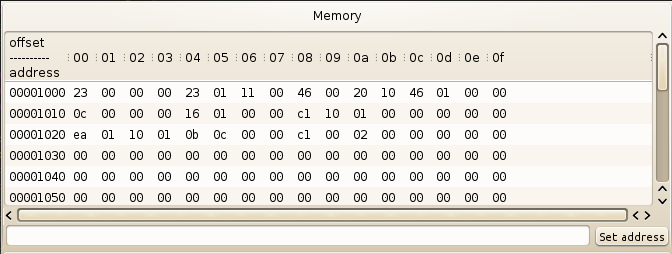
\includegraphics[width=0.8\textwidth]{./files/emu_gui_mem_memory.png}
\end{center}
	\caption{The physical memory from address 0x00001000.}
\end{figure}

\subsection{Panel Cache}
The cache panel lets you inspect each cache line. Just enter the cache line number in the input field below and press \emph{enter} and the desired cache line is displayed.
\begin{figure}[H]
\begin{center}
	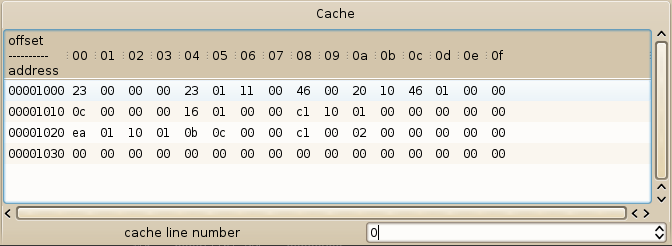
\includegraphics[width=0.8\textwidth]{./files/emu_gui_mem_cache.png}
\end{center}
	\caption{The cached contents of cache line zero are displayed.}
\end{figure}